%! suppress = MissingImport
%! Author = maxwe
%! Date = 10.03.22

% Preamble
\documentclass[11pt]{PyRollDocs}

\addbibresource{refs.bib}

\newmintinline[py]{python}{}

% Document
\begin{document}

    \title{The Pillar Model PyRoll Plugin}
    \author{Max Weiner}
    \date{\today}

    \maketitle

    The Pillar Model plugin serves as a base package for other plugins using the division of the profile in collinear pillars along width direction.
    It is mainly intended for calculation of material flow, groove filling and spread.


    \section{Model Approach}\label{sec:model-approach}

    \subsection{Discretization of Profile Cross-Sections}\label{subsec:discretization-of-profile-cross-sections}

    \begin{figure}
        \centering
        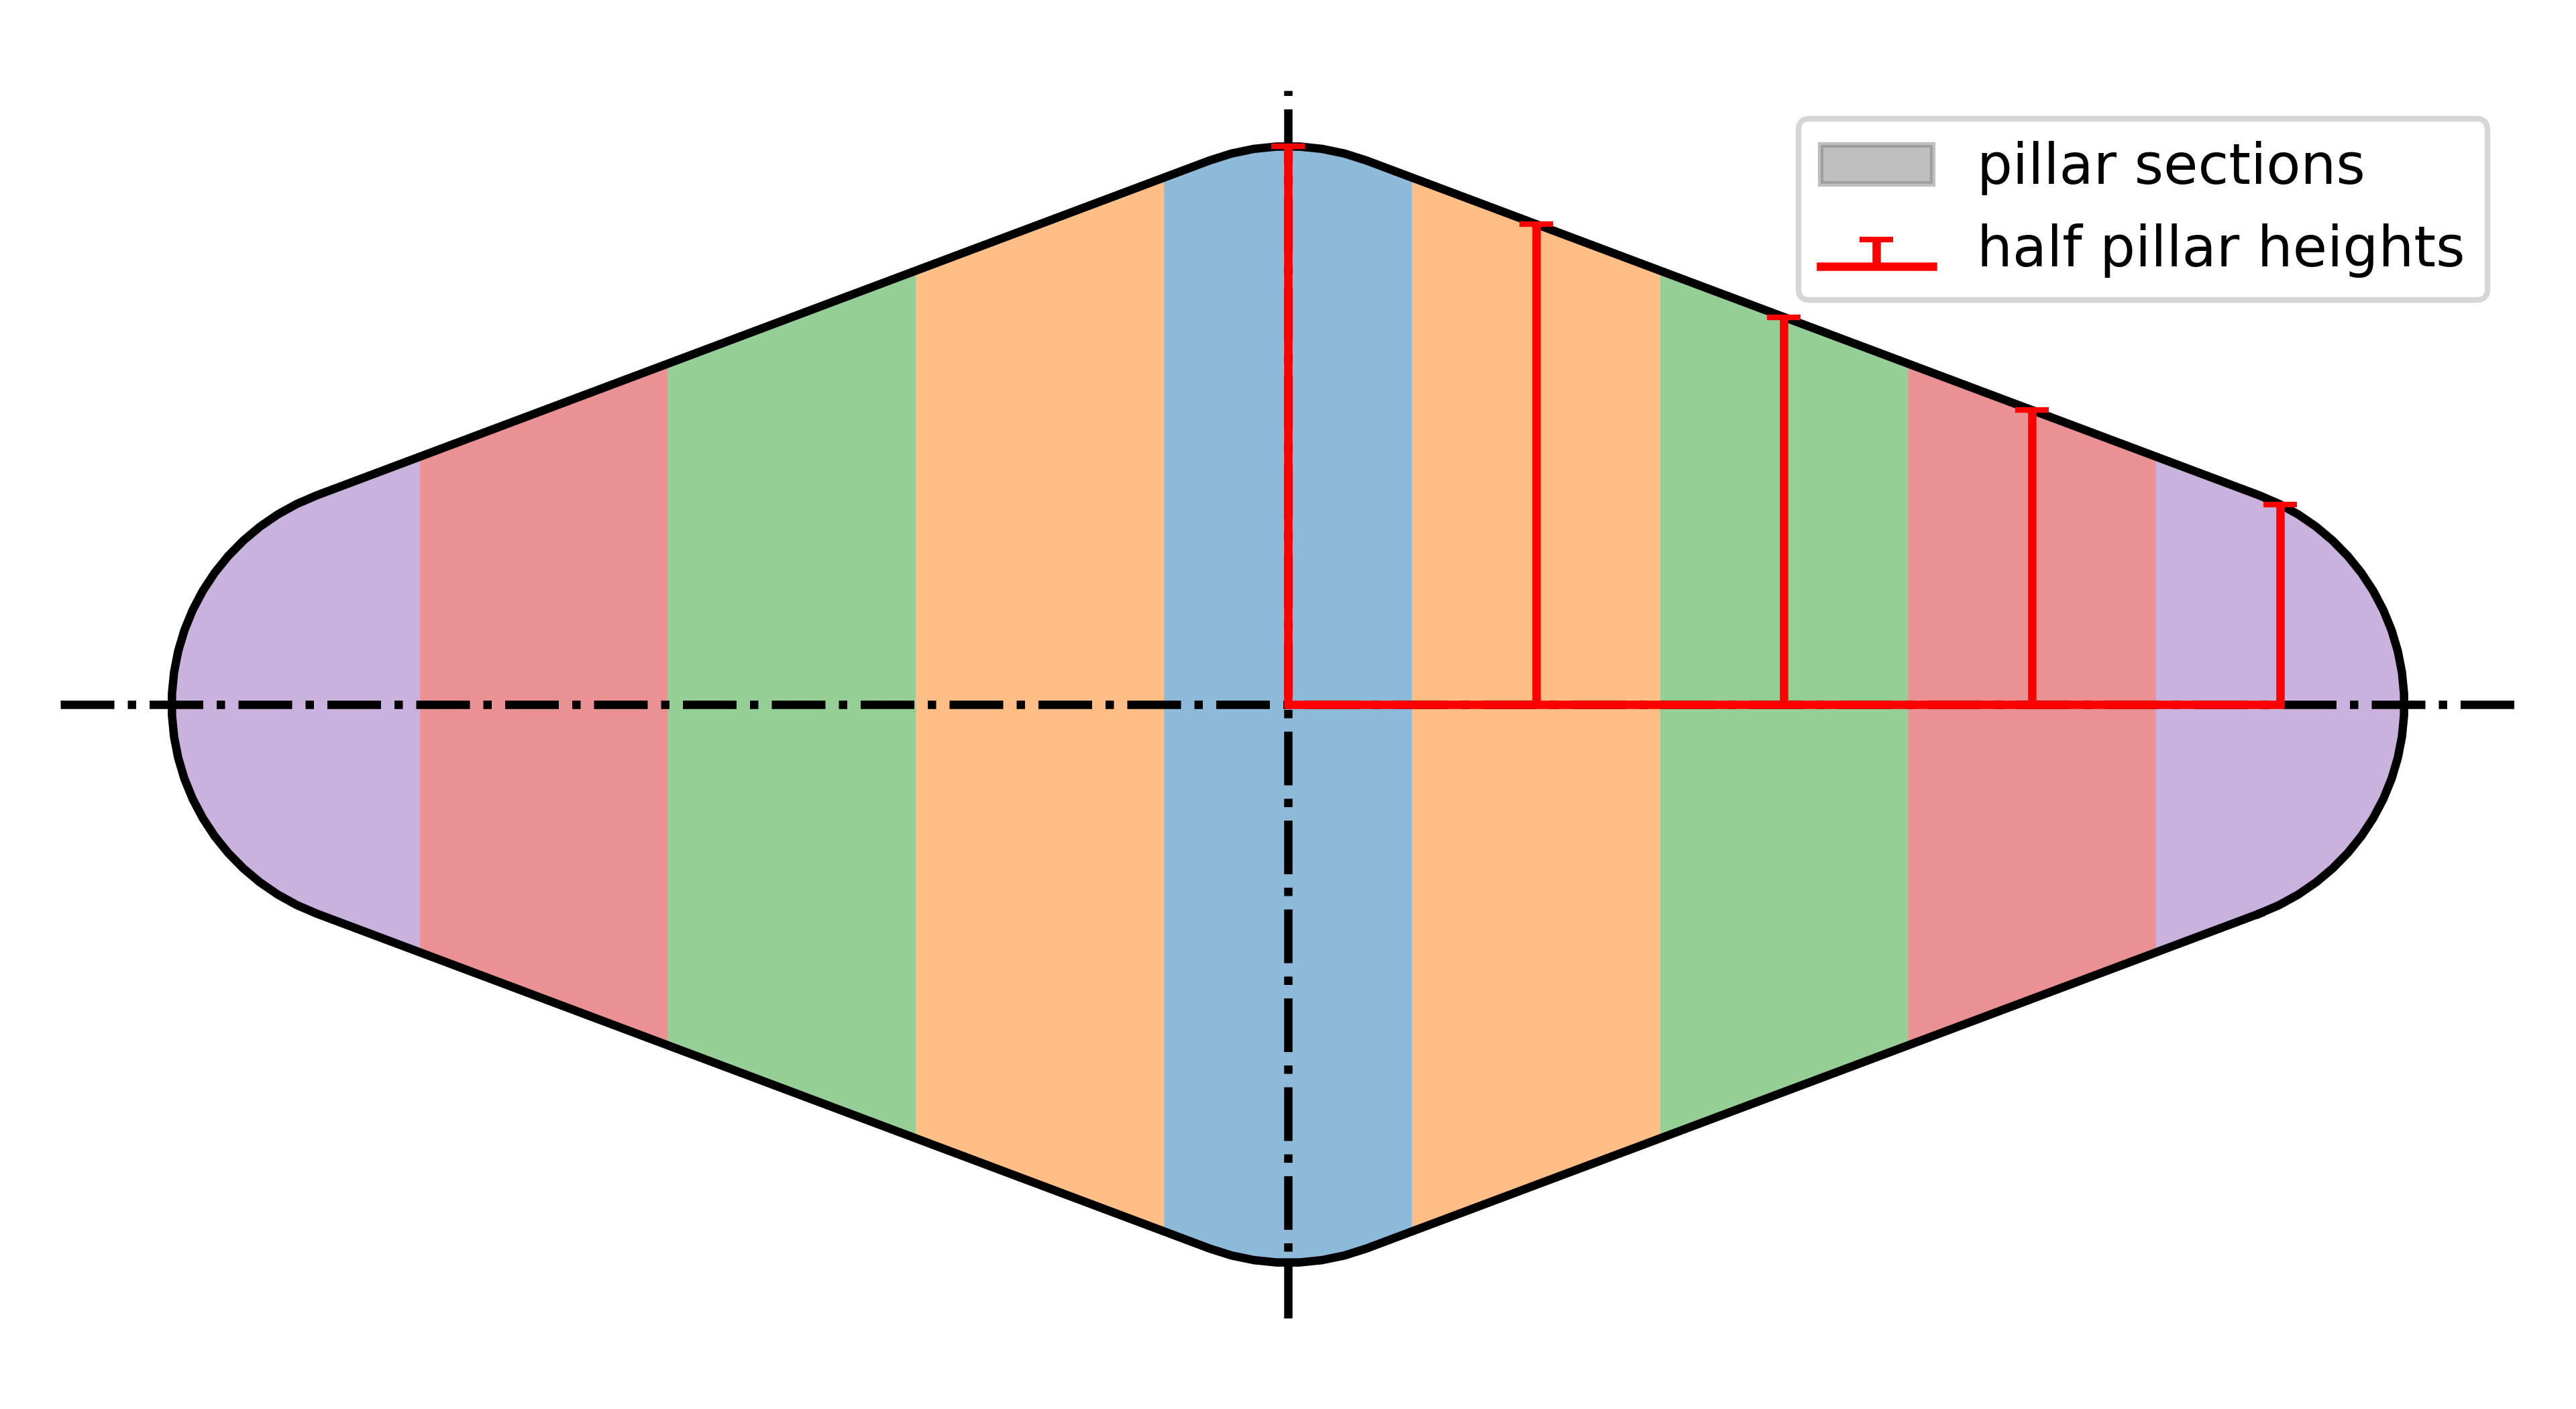
\includegraphics[width=0.6\linewidth]{img/pillar_profile}
        \caption{Example of Pillar Discretization for a Diamond Profile With 5 Pillars (Symmetrical)}
        \label{fig:pillar_profile}
    \end{figure}

    The pillar model introduces a discretization of the profile cross-section into distinct pillars as shown in \autoref{fig:pillar_profile}.
    The pillars' positions are defined by their center points $z_i$.
    $i \in [0, n - 1]$ is the index of the pillar, with $n$ as the count of pillars.
    Each pillar has a defined width $w_i$ and height $h_i$.
    The height is always measured at $z_i$.

    When discretizing an existing profile, the $z_i$ are calculated as in \autoref{eq:pillars}, with $w$ as the maximum profile width.
    However, during deformation the positions may change, so one shall not depend on equidistant pillars.

    \begin{equation}
        z_i = i \Delta z
        \qquad\text{with}\
        \Delta z = \frac{w}{n - \frac{1}{2}}
        \label{eq:pillars}
    \end{equation}

    The boundaries $Z_j$ with $j \in [0, n]$ of the pillars are located halfway between their positions, but the innermost boundary is identical with the position $z_0 = Z_0 = 0$.

    \begin{equation}
        Z_j = \frac{z_j - z_{j-1}}{2}
        \label{eq:pillar_boundaries}
    \end{equation}

    The pillar widths $w_i$ are defined as the distance between their boundaries.
    Note, that the numerical width of the inner pillar $w_0$ is initially the half of the others due to $z_0 = Z_0 = 0$.

    \begin{equation}
        w_i = Z_{i+1} - Z_i
        \label{eq:pillar_widths}
    \end{equation}

    \subsection{Pillar Behavior in Roll Passes}\label{subsec:pillar-behavior-in-roll-passes}

    \begin{figure}
        \centering
        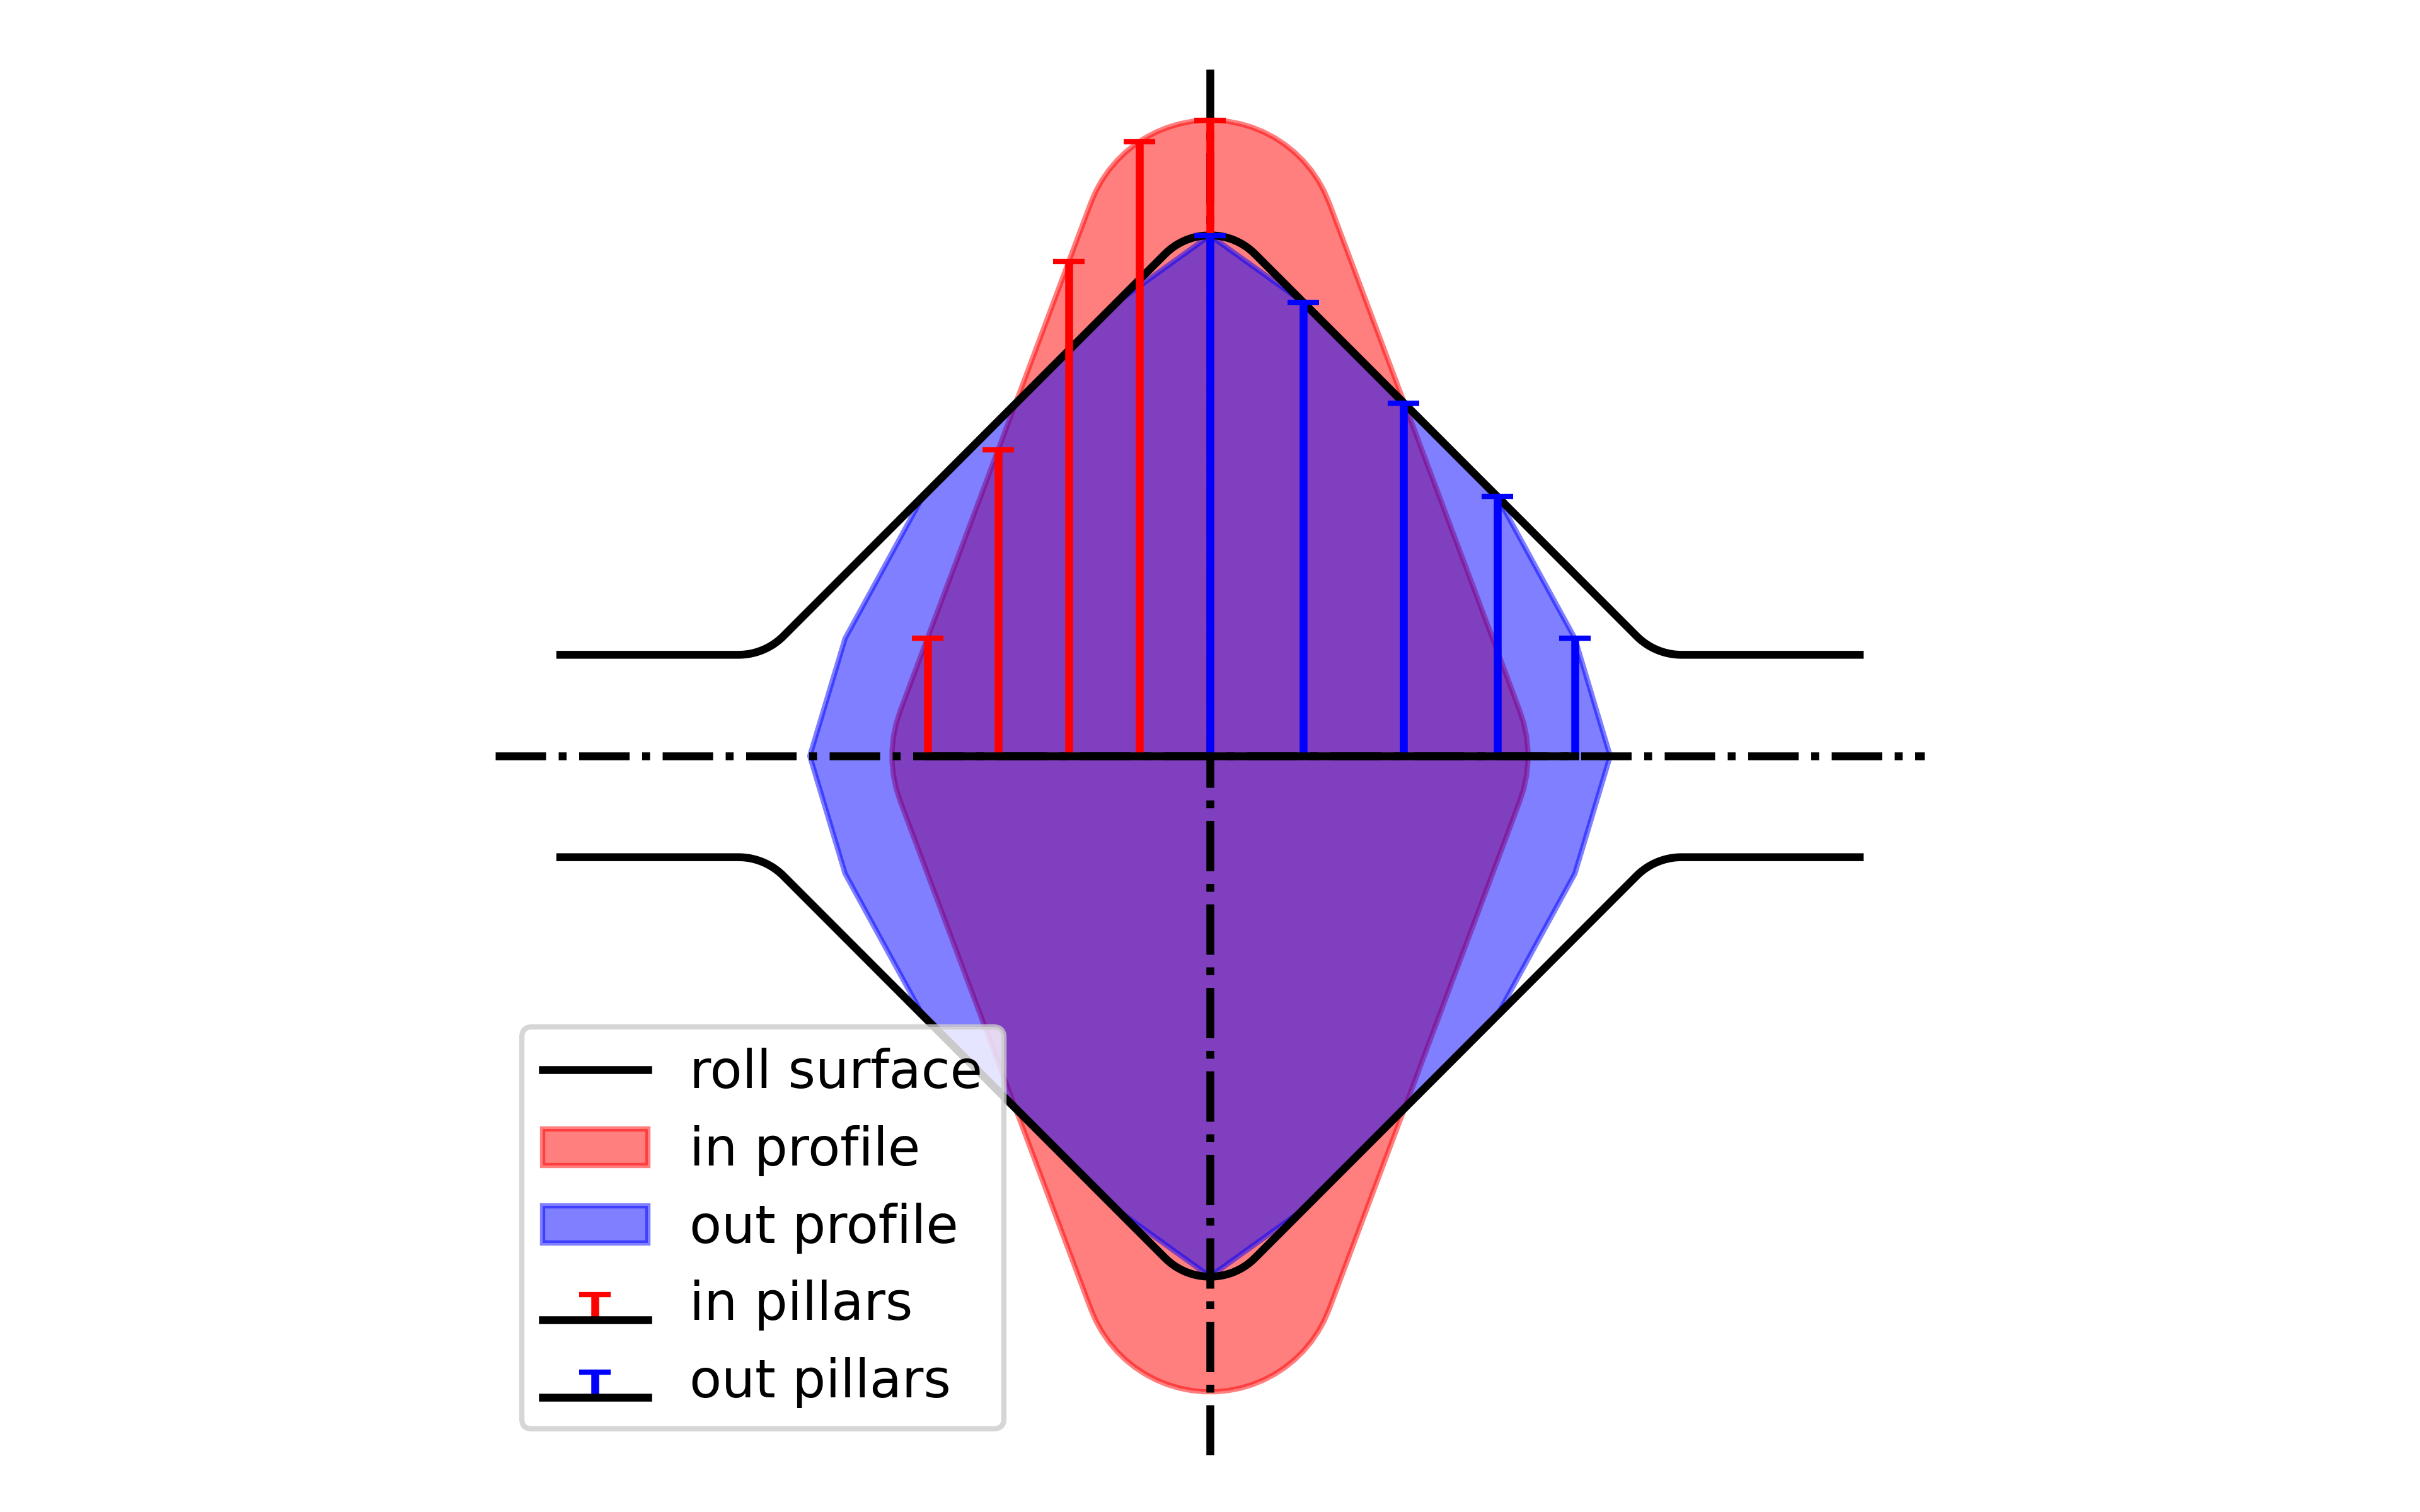
\includegraphics[width=0.6\linewidth]{img/pillar_disk_element}
        \caption{Deformation of a Pillared Profile in a Disk Element of a Roll Pass}
        \label{fig:pillar_disk_element}
    \end{figure}

    The main purpose of the pillar model is to model geometry evolution in the disk elements of roll passes.
    In the following, the upper indizes $0$ and $1$ denote the incoming resp. outgoing profile's values.

    \autoref{fig:pillar_disk_element} shows the intended deformation of a pillar-discretized profile within a roll pass disk element.
    Note, that the spreading in the figure is heavily exagerated for illustration purpose.

    The incoming profile shows here a smooth surface, as it was generated by \py/Profile.diamond()/, the same way as the profile in \autoref{fig:pillar_profile}.
    The outgoing profile has lost its smooth surface, since the cross-section shape can only be described by the use of the pillars positions $z_i^1$ and heights $h_i^1$, so the cross-section becomes a linear line string.
    Additional points are added at $(Z_n, 0)$ and $(-Z_n, 0)$ to provide a senseful outer boundary and ensure consistency with the pillar creation described above.
    Note, that only the pillars 1--3 (from center to side) are here in contact with the roll surface, as their height is larger than the local roll pass height.
    Only they are experiencing deformation, with reduction in height and increase in width.
    The other pillars are shifted to the outside according to the others' widths, but maintain their heights.

    The new pillar widths $w_i^1$ are calculated using their spread $\beta_i$. $\beta_i$ defaults to \num{1}, actual implementations are deferred to other plugins.

    \begin{equation}
        w_i^1 = \beta_i w_i^0
        \label{eq:spread}
    \end{equation}

    The new boundaries result from this in a cumulative way as:

    \begin{equation}
        Z_{j+1}^1 = Z_j^1 + w_j \qquad \text{with}\ Z_0^1 = 0
        \label{eq:boundaries1}
    \end{equation}

    And therefore the pillar position $z_i^1$ as:

    \begin{equation}
        z_i^1 = \frac{Z^1_{i+1} - Z^1_i}{2}
        \label{eq:pillars1}
    \end{equation}


    \section{Usage Instructions and Implementation Details}\label{sec:usage-instructions}

    Packages residing on this type of discretization shall depend on this plugin to create a common interface.
    In the following, the hooks defined by this plugin shall be described, and instructions shall be given, how to implement model equations for specific purposes.

    The pillar model plugin defines hooks on \py/pyroll.core.Profile/ for the purpose of pillar representation and initial creating as described in \autoref{subsec:discretization-of-profile-cross-sections}.
    The central hook of this package is \py/Profile.pillars/.
    It returns a numpy array of the $z$ coordinates representing the centers of the pillars acc.\ to \autoref{eq:pillars}.
    The respective pillar boundaries' coordinates acc.\ to \autoref{eq:pillar_boundaries}  are provided by the \py/Profile.pillar_boundaries/ hook.
    The heights $h_i$ are provided by the \py/Profile.pillar_heights/ hook, as the widths by the \py/Profile.pillar_widths/ hook.
    General implementations of these hooks are provided according to \autoref{eq:pillars}, \autoref{eq:pillar_boundaries} and \autoref{eq:pillar_widths}.
    The heights are determined by intersection of the profiles cross-section polygon with vertical lines at the respective $z_i$.
    Polygons representing the pillars are provided by the \py/Profile.pillar_sections/ hook, obtained by clipping the profile's cross-section.

    To modify the initial pillar distancing, provide a new implementation of \py/Profile.pillars/.
    Users of this plugin must not not rely on equidistant pillars, but calculate needed distances from the respective coordinates.
    Especially in roll passes the pillar posotions \emph{will} change due to spreading calculation, if an respective plugin is loaded additionally.

    Reagrding the behavior of pillars in roll passes the following hooks are defined:
    \begin{description}
        \item[\py/RollPass.DiskElement.pillars_in_contact/] returns a boolean array indicating which pillars have contact to the roll surface in this disk element.
        \item[\py/RollPass.DiskElement.pillar_spreads/] returns an array with the pillars' spreads $\beta_i$. Defaults to ones for all pillars.
        \item[\py/RollPass.DiskElement.pillar_draughts/] returns an array with the pillars' draughts $\gamma_i$. Defaults to $h_i^1 / h_i^0$.
        \item[\py/RollPass.DiskElement.pillar_spreads/] returns an array with the pillars' elongations $\lambda_i$. Defaults to $(\beta_i\gamma_i)^{-1}$.
    \end{description}

    Implementations of the profile hooks above on \py/RollPass.DiskElement/ are provided following the procedure in \autoref{subsec:pillar-behavior-in-roll-passes}.

    Plugins aiming at spread calculation using the pillar approad should provide an implementation of \py/RollPass.DiskElement.pillar_spreads/ yielding the respective values.
    Users of PyRolL (non-developers) generally do not need to provide anything for usage of this plugin, except they may set the \py/pyroll.pillar_model.PILLAR_COUNT/ constant to a desired value.
    The value must be a non-negative integer, it is explicitly recommended to not change this during simulation runs, as it may corrupt data already generated.

    For implementing additional model equations, define a new hook \py/Profile.pillar_*s/ which shall return an array of the same length as \py/Profile.rings/.
    The \texttt{*} shall be replaced with the property name you want to represent, pay respect to the plural form.
    For hooks on units or disk elements act respectively.

    \printbibliography

\end{document}